\documentclass[../DS05.tex]{subfiles}
\graphicspath{{./figures/}}

% \subimport{/home/nora/Documents/Enseignement/Prepa/bpep/exercices/DS/ondes_gravitationnelles/}{sujet.tex}
\begin{document}

\exercice[26]{Ondes gravitationnelles}
\enonce{
	Le prix Nobel 2017 a été remis aux responsables de l'expérience Ligo, qui a détecté des ondes gravitationnelles trois fois en un an. Cette expérience n'est pas la seule dans le monde. L'expérience franco-italienne Virgo a également détecté cette même année et pour la première fois des ondes gravitationnelles. Ces expériences exploitent le phénomène d'interférences lumineuses.
  \smallbreak
  \noindent
  \begin{minipage}[c]{.54\linewidth}
    ~
    \begin{center}
      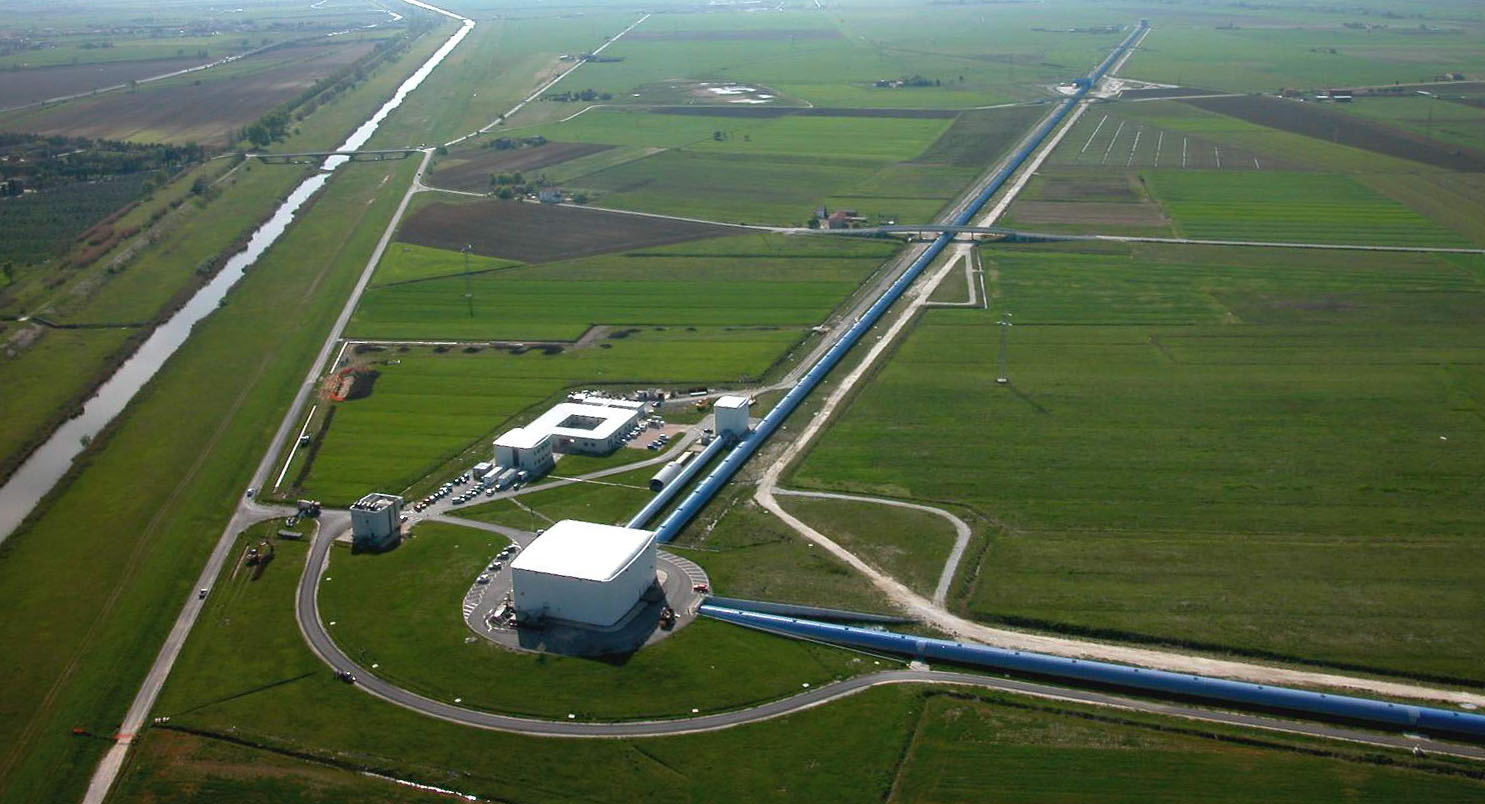
\includegraphics[width=\linewidth]{virgo}
      \captionof{figure}{Photo aérienne de l'interféromètre Virgo}
    \label{fig:virgo}
    \end{center}
  \end{minipage}
  \hfill
  \begin{minipage}[c]{.45\linewidth}
    ~
    \begin{center}
      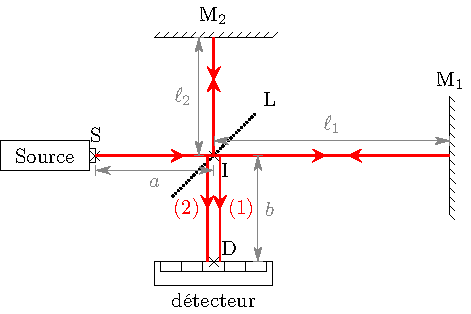
\includegraphics[width=\linewidth]{virgo_inter}
      \captionof{figure}{Photo aérienne de l'interféromètre Virgo}
    \label{fig:virgo_inter}
    \end{center}
  \end{minipage}

   Une source laser de longueur d'onde $\lambda = \SI{633}{\nano\meter}$ se
   trouve au point S et émet un faisceau de lumière le long de l'axe $(Ox)$. Ce
   faisceau laser est séparé en deux par une lame séparatrice L. On considère
   alors que la moitié de la lumière entre dans le bras 1 et l'autre moitié
   dans le bras 2. Chaque faisceau ainsi obtenu parcourt un bras de
   l'interféromètre, est réfléchi sur un miroir (M$_1$ ou M$_2$) et revient vers
   la séparatrice.
   \bigbreak
  Le faisceau est recombiné par la séparatrice et le signal résultant est
  détecté par le détecteur D. La source laser émet au point S un signal de la
  forme $A \cos (\omega t)$. Les deux bras de l'interféromètre ont pour longueur
  respectives $\ell_1$ et $\ell_2$. La distance entre la source S et la
  séparatrice est noté $a$ et la distance entre la séparatrice et le détecteur
  D est notée $b$.
	\bigbreak
  On négligera toute diminution de l'amplitude de l'onde lumineuse au cours de
  sa propagation (sur la Figure~\ref{fig:virgo_inter}, les rayons incidents et
  réfléchis sont décalés dans les bras de l'interféromètre pour améliorer la
  lisibilité de la figure~; en pratique, les rayons sont superposés).
}


\QR{
  Calculer la distance parcourue par le rayon qui effectue le parcours (SD)$_1$
  se réfléchissant sur M$_1$ en fonction de $a$, $\ell_1$ et $b$.
}{
  \[
    \boxed{
      ({\rm SD})_1 =
      ({\rm SI}) + ({\rm IM_1}) + ({\rm M_1I}) + ({\rm ID}) = 
      a+2\ell_1 + b
    }
  \]
}

\QR{
	En déduire l'expression du signal $s_1$ au point $D$ de l'onde lumineuse ayant effectuée le parcours (SD)$_1$.
}{
  Le signal met une durée $\Delta t_1=(a+2\ell_1 + b)/c$ pour aller de la source
  au détecteur. De plus, la moitié du signal est perdu à chaque fois que le
  faisceau traverse la lame semi-réfléchissante. Finalement
  \[
        s_1(t) =
        \frac{A}{4}\cos(\omega (t- \Delta t_1) ) =
        \frac{A}{4}\cos(\omega (t- (a+2\ell_1 + b)/c) ) =
        \boxed{\frac{A}{4}\cos(\omega t- \frac{2\pi}{\lambda} (a+2\ell_1 + b))}
  \]
}

\QR{
	Calculer la distance parcourue par le rayon qui effectue le parcours $E \to I \to M_2 \to I \to D$ en fonction de $a$, $\ell_2$ et $b$.
}{
	\eq{
		\boxed{E \to I \to M_2 \to I \to D=a+2\ell_2 + b}
	}

}


\QR{
	En déduire l'expression du signal $s_2$ au point $D$ de l'onde lumineuse ayant effectuée le parcours $E \to I \to M_2 \to I \to D$.
}{
	\eq{
		\boxed{s_2(t)=\frac{A}{4}\cos(\omega t- 2\pi (a+2\ell_2 + b)/\lambda )}.
	}

}

\enonce{
	\noindent On rappelle la formule d'addition :
	\eq{
		\cos a + \cos b = 2\cos \left( \frac{a+b}{2} \right) \cos\left( \frac{a-b}{2} \right).
	}

}


\QR{
	Montrer que le signal lumineux total $s(t) = s_1(t) + s_2(t)$ mesuré par le détecteur au point $D$ est :
	\eq{
		s(t) = \frac{A}{2}\left[
			\cos\left(\omega t- 2 \pi \times \frac{a+\ell_1 + \ell_2+ b}{\lambda} \right)
			\times \cos\left(\frac{2\pi}{\lambda} (\ell_2-\ell_1)  \right)\right].
	}

}{
	\begin{align*}
		s(t)=\frac{A}{4}\left(
		\cos\left(\omega t- 2\pi \frac{a+2\ell_1 + b}{\lambda} \right)
		+
		\cos\left(\omega t- 2\pi \frac{a+2\ell_2 + b}{\lambda}\right)\right)
		\\
		=\frac{A}{2}\left(
		\cos\left(\omega t- \pi \frac{a+2\ell_1 + b}{\lambda} - \pi \frac{a+2\ell_2 + b}{\lambda}\right)
		\times \cos\left(- \pi \frac{a+2\ell_1 + b}{\lambda} +  \pi \frac{a+2\ell_2 + b}{\lambda} \right)\right)
		\\
		=\frac{A}{2}\left(
		\cos\left(\omega t- 2 \pi \frac{a+\ell_1 + \ell_2+ b}{\lambda} \right)
		\times \cos\left(\frac{2\pi}{\lambda} (\ell_2-\ell_1)  \right)\right)
	\end{align*}
}


\QR{
	Proposer une condition sur $\ell_1$ et $\ell_2$ pour que les deux signaux $s_1$ et $s_2$ soient en quadrature de phase au niveau du détecteur, c'est-à-dire déphasés de $\pi/2$.
}{
	\eq{
		\frac{2\pi(2\ell_1-2\ell_2)}{\lambda} = \frac{\pi}{2}
		\qquad \Rightarrow \qquad
		\boxed{\ell_1-\ell_2=\frac{\lambda}{8}}.
	}

}

\enonce{
	\noindent Lors du passage d'une onde gravitationnelle, les bras de l'interféromètre se déforment. Les longueurs $\ell_1$ et $\ell_2$ varient alors en fonction du temps.
}


\QR{
	Expliquer comment cet interféromètre permet de détecter le passage d'une onde gravitationnelle. \\ Qu'observe-t-on au niveau du détecteur ?
}{
	Quand il y a une onde gravitationnelle, les longueurs $\ell_2$ et $\ell_1$ ne varient pas de la même façon. Donc $(\ell_1-\ell_2)$ varie. On voit donc une variation du signal en $D$ qui est maximum quand les 2 ondes sont en phase (interférence constructives) et minimale quand les 2 ondes sont en opposition de phase (interférences destructives).
}



\end{document}
